% $Id$

\subsection{\label{ssec:high-arch}High-level \emph{vic} Architecture}

We have drawn a high-level overview \emph{vic} architecture (sender only) that
has congestion control modules as in Figure~\ref{fig:high-arch}. This figure
represents a high-level overview of \emph{vic} so that we could see the major
components of the system, and how they are interacting with each other. 

\vspace{1cm}

\begin{figure}[!h]
\begin{center}
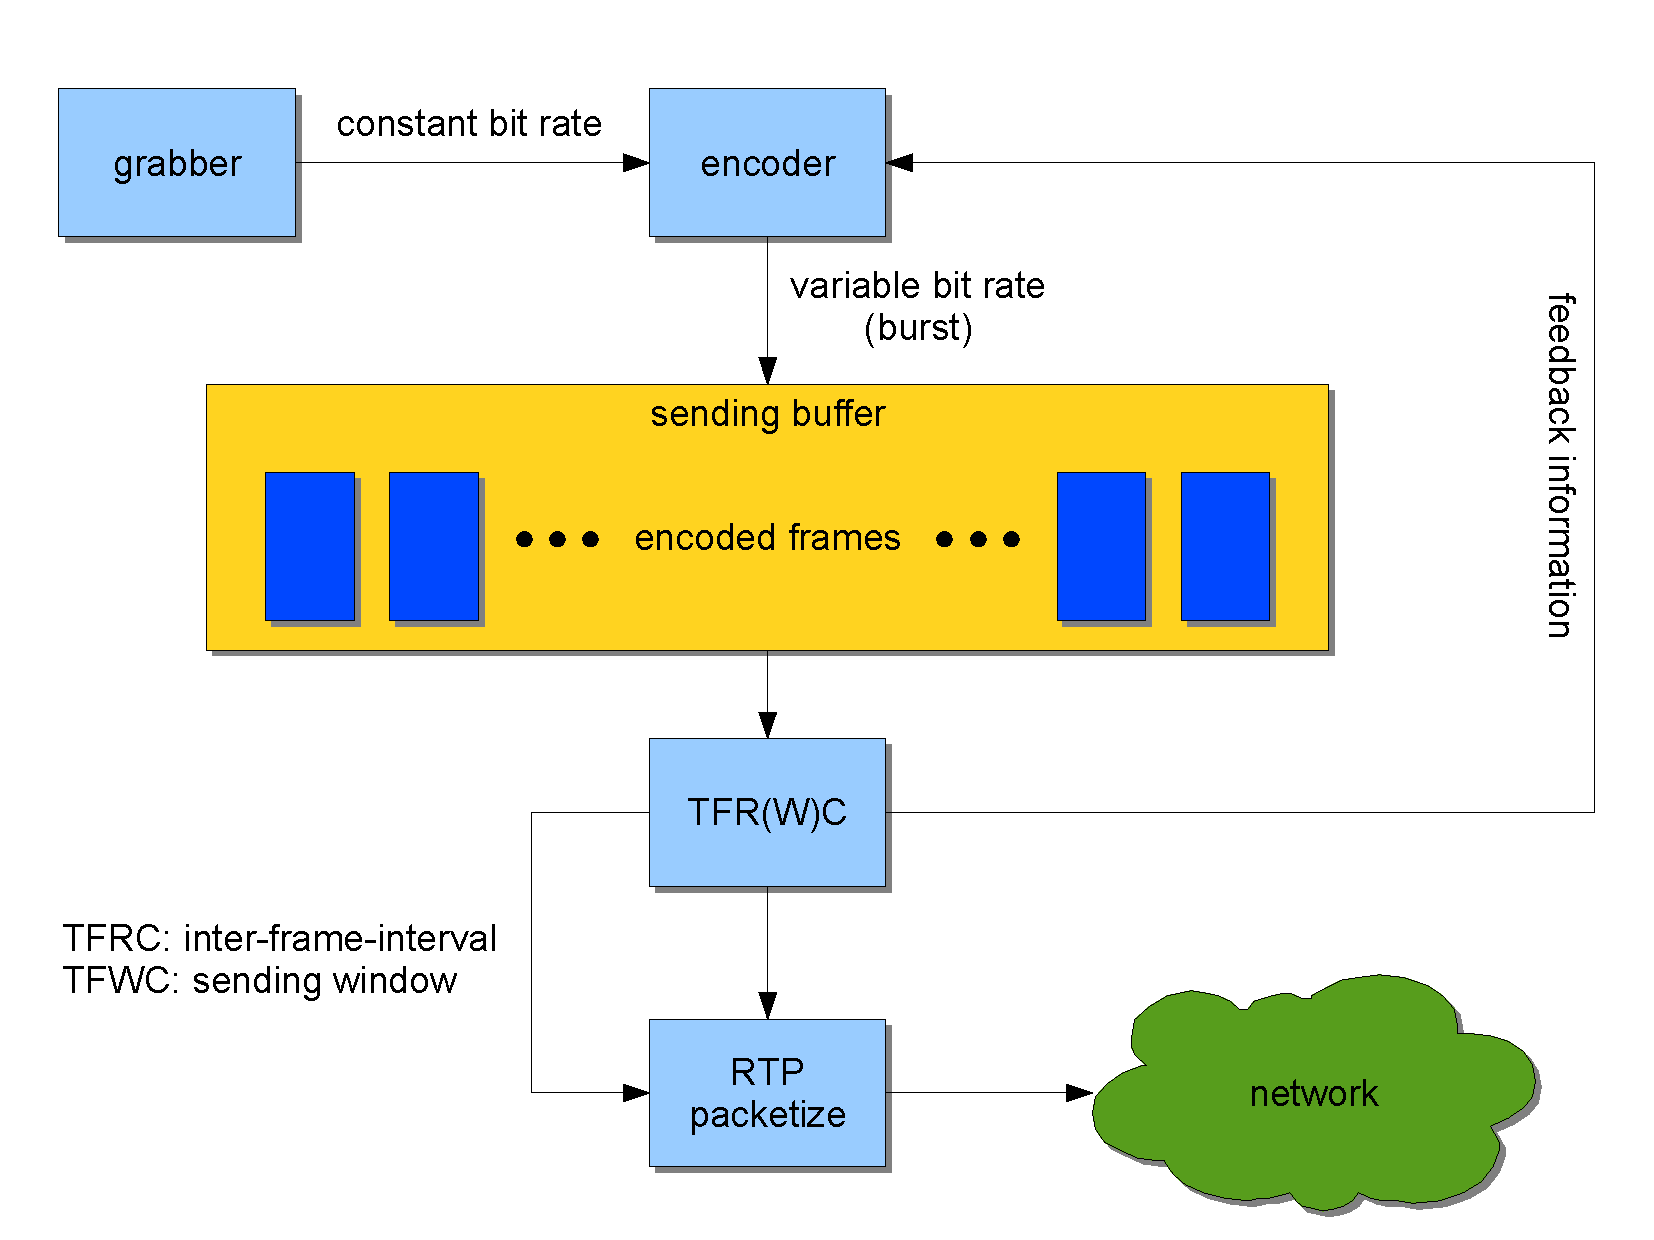
\includegraphics[scale=.5]{./img/high-vic-arch}
\caption{\label{fig:high-arch}High-level Overview \emph{vic} Architecture 
with CC Mechanisms}
\end{center}
\end{figure}

Unlike to the sender, we envisage the architecture of the receiver is relatively
simple. For example, upon a packet reception, it will be inserted to a receive
buffer, subsequently decoded (and some color conversion if necessary), and
finally displayed in a output device. Depending upon a codec, the rendered
frames may not be discareded immediately, but will be kept for some times before
they get purged.

\newpage
